\subsubsection{Incremento 13}
\textit{\textbf{Periodo}: dal 2021-05-13 al 2021-05-26}

\myparagraph{Obiettivi}
Gli obiettivi definiti per questo incremento sono i seguenti:
\begin{itemize}

\item preparazione alla presentazione della Revisione di Accettazione;
\item preparazione al collaudo finale con il proponente;
\item incremento della documentazione.
\end{itemize}

\myparagraph{Attività}
Per raggiungere gli obiettivi, vengono svolte le seguenti attività:
\begin{itemize}
\item \textbf{presentazione Revisione di Accettazione}: creazione e preparazione della presentazione con il \VT{};
\item \textbf{collaudo}: controlli e verifiche ultime al prodotto e ai documenti per il collaudo finale con il proponente;
\item \textbf{ampliamento documentazione e verifiche}:
\begin{itemize}
\item incremento del \Glossariov{3.0.0};
\item rilevazione e registrazione di metriche, esiti di verifica e obiettivi di qualità;
\item aggiornamento dei rischi rilevati;
\item calcolo e registrazione del consuntivo di periodo.
\end{itemize}

\end{itemize}
\myparagraph{Diagramma di Gantt}
\begin{figure}[H]
\centering

\centerline{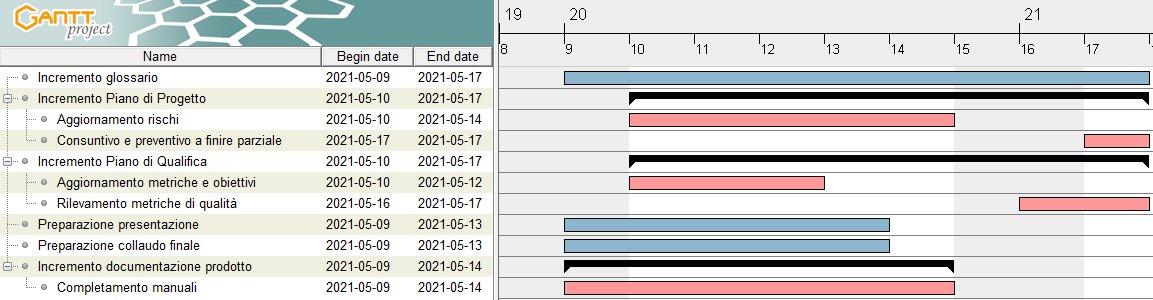
\includegraphics[scale=0.6]{res/Pianificazione/Fasi/VerificaIncrementi/ganttIncremento13}}
\caption{Diagramma di Gantt per l'incremento 13}
\end{figure}